\subsection{Constraints on possible pointing strategies}
\label{sec:constraints_on_pointings}

The spacecraft has finite fuel reserves for necessary maneuvers, but
the reserves are expected to last about 10 years [R. Vanderspek,
  priv. comm.], well past the three-year time horizon that is the
focus of this study.

When considering possible schedules for telescope pointings, the main
constraint is that the cameras must be directed approximately opposite
the Sun.  Specifically, the center of the combined fields-of-view is
ideally pointed within 15$^\circ$ of the antisolar direction, and no
more than 30$^\circ$ away.
%\todo[inline]{Roland: are these numbers still good? are they imposed by the sunshade? or solar panels? Some comment appreciated.} 
This is necessary for the sunshade and spacecraft to block solar
photons.  It also enables the solar panels (which are free to rotate
about the $+Y$ axis in Fig.~\ref{fig:spacecraft_angles}) to collect
sunlight.  Given the spacecraft's orbit~\citep{gangestad_high_2013},
this means that \tess should advance $\sim28^\circ$ east in ecliptic
longitude every lunar month, as it does during the Primary Mission.
Focusing on a fixed field for say, 3 spacecraft orbits ($\approx$42
days), would be in tension with this requirement.  In practice,
another technical restriction is whether the Earth or Moon passes
through \tesss camera fields during a proposed pointing (see
Sec.~\ref{sec:earth_moon_crossings}).

\begin{figure}[!b]
	\centering
	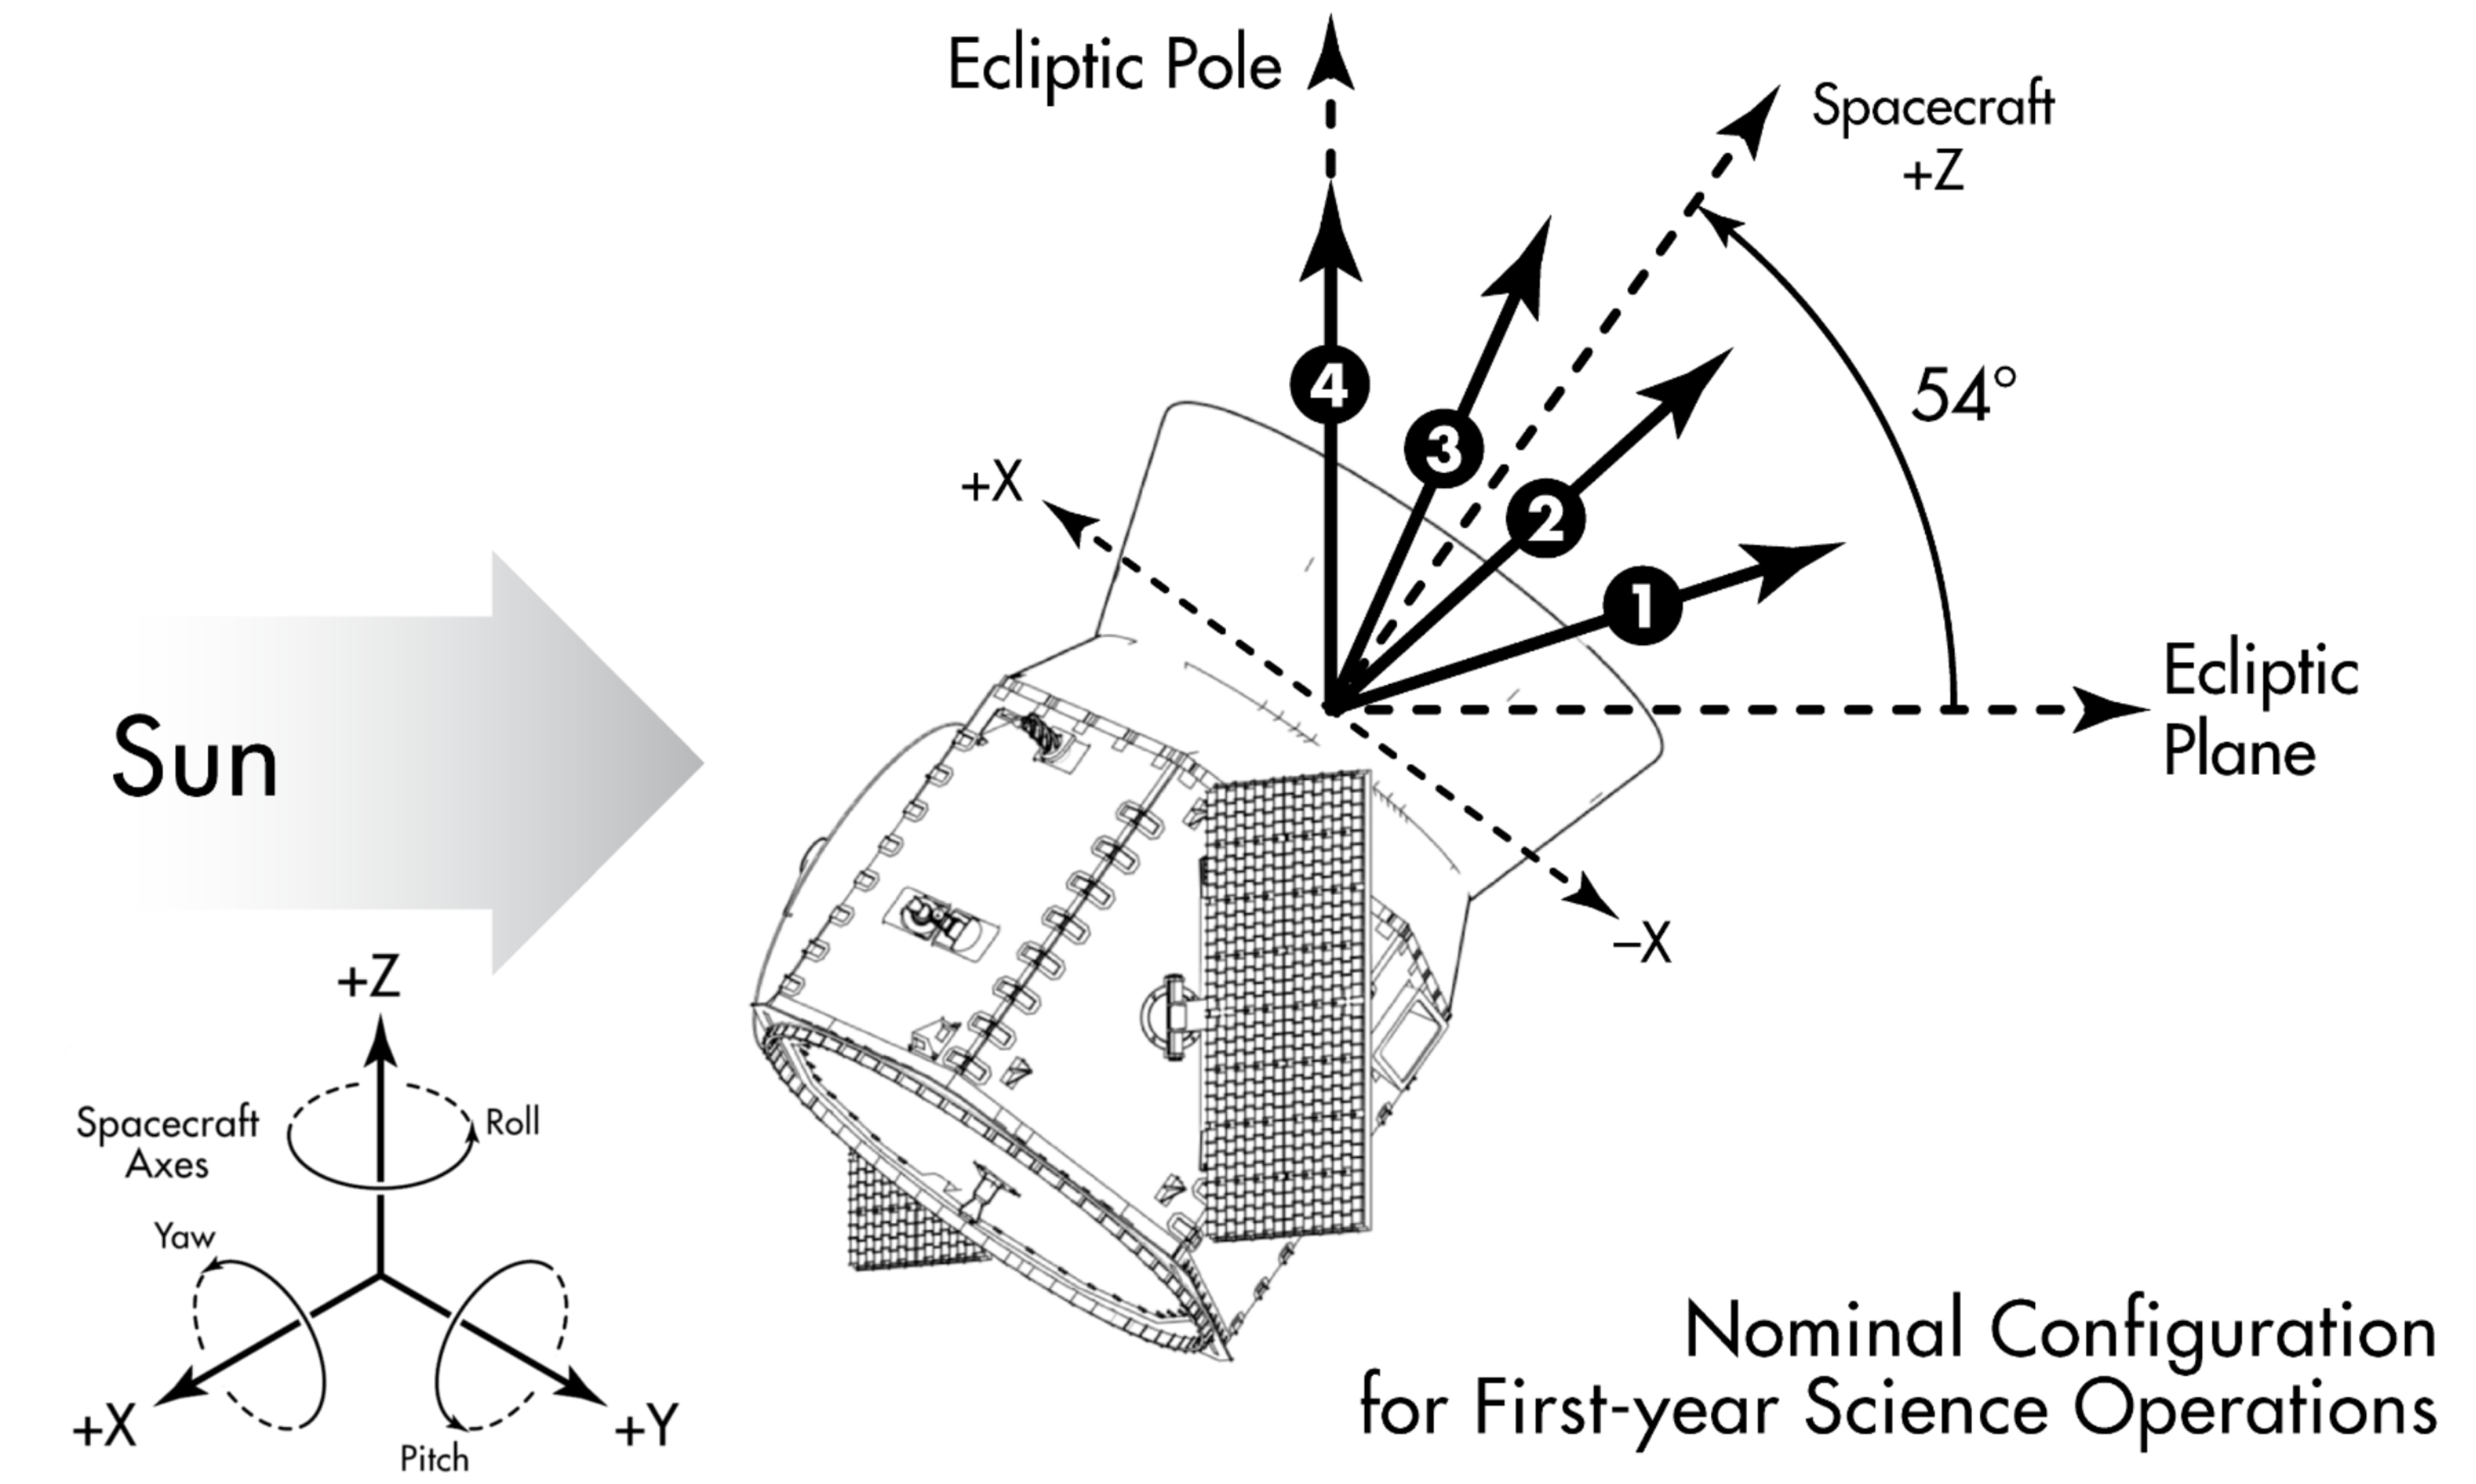
\includegraphics{figures/spacecraft_angles.pdf}
	\caption{\tesss solar panels pitch about the $+Y$ axis. The spacecraft must point so that incident sunlight is collected by the solar panels, and not the cameras. (Adapted from Orbital ATK design document) }
	\label{fig:spacecraft_angles}
\end{figure}
